			\section*{Exercice 4 (5 points)}			
			\subsection*{1. Déterminer le coût moyen quotidien pour la production de 5 m$^3$ d’engrais.}
			
			On a :
			\[
			f(5) = \dfrac{5^2 - 15 \times 5 + 400}{5} = \dfrac{25 - 75 + 400}{5} = \dfrac{350}{5} = 70
			\]
			
			Le coût moyen de 5 m$^3$ d’engrais est 7 000 €.
			
			\subsection*{2. Quels volumes d’engrais faut-il fabriquer pour avoir un coût moyen de production égal à 4 300 € (43 centaines d’euros) ?}
			
			Il faut résoudre l’équation :
			\[
			f(x) = 43 \iff \dfrac{x^2 - 15x + 400}{x} = 43 \iff x^2 - 15x + 400 = 43x \quad (avec \ x \neq 0)
			\]
			\[
			\iff x^2 - 58x + 400 = 0
			\]
			
			Avec $\Delta = 58^2 - 4 \times 400 = 3364 - 1600 = 1764 = 42^2$, les racines sont :
			\[
			x_1 = \dfrac{58 + 42}{2} = 50 \quad \text{et} \quad x_2 = \dfrac{58 - 42}{2} = 8
			\]
			
			En fabriquant 8 ou 50 m$^3$ d’engrais le coût moyen de production est 4 300 €.
			
			\subsection*{3. Pour quel volume d’engrais fabriqué le coût moyen de production est-il minimal ? Déterminer ce coût moyen minimal.}
			
			La fonction $f$ est dérivable sur $[5 ; 60]$ et sur cet intervalle :
			\[
			f'(x) = \dfrac{x(2x - 15) - (x^2 - 15x + 400)}{x^2} = \dfrac{2x^2 - 15x - x^2 + 15x - 400}{x^2} = \dfrac{x^2 - 400}{x^2} = \dfrac{(x + 20)(x - 20)}{x^2}
			\]
			
			$f'(x)$ est du signe de $(x + 20)(x - 20)$ (car $x^2 > 0$) et l’on sait que ce trinôme est positif sauf sur $] - 20 ; 20[$.
			
			Donc sur $[5 ; 20[$, $f'(x) < 0$ et $f$ est donc décroissante et sur $[20 ; 60]$, la fonction $f$ est croissante. \\
			D’où le tableau de variations (avec $f(20) = 25$) :
			\begin{center}
			\begin{tikzpicture}[double distance=2pt]
				\tkzTabInit{$x$/1,$f'(x)$/1,$f(x)$/2}{$5$,$20$, $60$}
				\tkzTabLine{,-,z, +}
				\tkzTabVar{+/$70$,-/$25$, +/$\alpha$}
			\end{tikzpicture}
		\end{center} 
			avec $\alpha=f(60)\approx51,7$\\
			D’après cette étude le minimum est atteint pour $x = 20$ et ce coût moyen minimal est égal à $f(20) = 25$, soit 2 500 €.
			
